% The sequence 1/n in the non-compact set (0,1]: every subsequence runs out to the missing point 0.
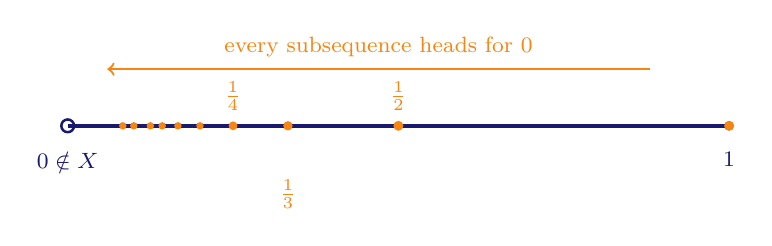
\begin{tikzpicture}[x=8.4cm,y=1cm,every node/.style={font=\footnotesize}]
  \draw[MidnightBlue,line width=1.3pt] (0,0) -- (1,0);
  \draw[MidnightBlue,line width=0.9pt] (0,0) circle (2.3pt);
  \fill[MidnightBlue] (1,0) circle (1.7pt);
  \node[below=6pt,MidnightBlue] at (0,0) {$0\notin X$};
  \node[below=6pt,MidnightBlue] at (1,0) {$1$};
  % Terms 1, 1/2, ..., 1/12. The first term is the closed endpoint.
  \fill[BurntOrange] (1,0) circle (1.8pt);
  \fill[BurntOrange] (0.5,0) circle (1.8pt);
  \node[above=2pt,BurntOrange] at (0.5,0) {$\frac12$};
  \fill[BurntOrange] (0.333,0) circle (1.7pt);
  \node[below=16pt,BurntOrange] at (0.333,0) {$\frac13$};
  \fill[BurntOrange] (0.25,0) circle (1.6pt);
  \node[above=2pt,BurntOrange] at (0.25,0) {$\frac14$};
  \foreach \n in {5,6,7,8,10,12} {
    \fill[BurntOrange] ({1/\n},0) circle (1.35pt);
  }
  \draw[BurntOrange,->,thick] (0.88,0.72) -- (0.06,0.72);
  \node[above=1pt,BurntOrange] at (0.47,0.72) {every subsequence heads for $0$};
\end{tikzpicture}
